% Reduction-routes roadmap for the qp-diffusion paper (compact variant).
% Post-coincidence content (2026-07): BOTH microscopic routes fix A1 = (1,0)
% with the undressed longitudinal flux and conserved density N1*f; the branch
% route's moment reduction carries the spectral weight outside the divergence,
% and its BRT-dressed kernel gives N1*D_B = D_N.  C = (0,-1) is the legacy
% placement (Fick ansatz for f), not a route end point; the N1^2 dressing
% belongs to the transverse (charge) channel.  Build: pdflatex routes_roadmap.tex
\documentclass[tikz,border=6pt]{standalone}
\usepackage{amsmath,amssymb}
\usepackage{dsfont}
\usetikzlibrary{arrows.meta,positioning,calc}
\newcommand{\id}{\mathds{1}}

\definecolor{slate}{HTML}{2B3A55}
\definecolor{teal}{HTML}{00838F}
\definecolor{warmred}{HTML}{C0392B}
\definecolor{paleslate}{HTML}{E8ECF2}
\definecolor{paleteal}{HTML}{DCF0F2}
\definecolor{palered}{HTML}{FDECEA}

\newcommand{\DN}{D_{\mathrm N}}

\tikzset{
  base/.style={draw, rounded corners=4pt, align=center, inner sep=5pt,
    line width=0.8pt, font=\small},
  matrixbox/.style={base, draw=slate, fill=paleslate, text width=6.0cm},
  branchbox/.style={base, draw=warmred, fill=palered, text width=6.0cm},
  resultbox/.style={base, draw=teal, fill=paleteal, text width=7.2cm},
  legacybox/.style={base, draw=warmred, dashed, fill=white, text width=5.6cm,
    font=\scriptsize},
  notebox/.style={draw=slate!45, dashed, rounded corners=5pt, align=center,
    inner sep=6pt, line width=0.6pt, fill=white, font=\scriptsize,
    text width=13.6cm},
  arr/.style={-{Stealth[length=2.6mm]}, line width=0.9pt, slate},
  redarr/.style={-{Stealth[length=2.6mm]}, line width=0.9pt, warmred},
  reddash/.style={-{Stealth[length=2.6mm]}, line width=0.9pt, warmred, dashed},
  tealarr/.style={-{Stealth[length=2.6mm]}, line width=0.9pt, teal},
  lab/.style={font=\scriptsize\itshape, align=center, fill=white,
    inner sep=1.5pt},
}

\begin{document}
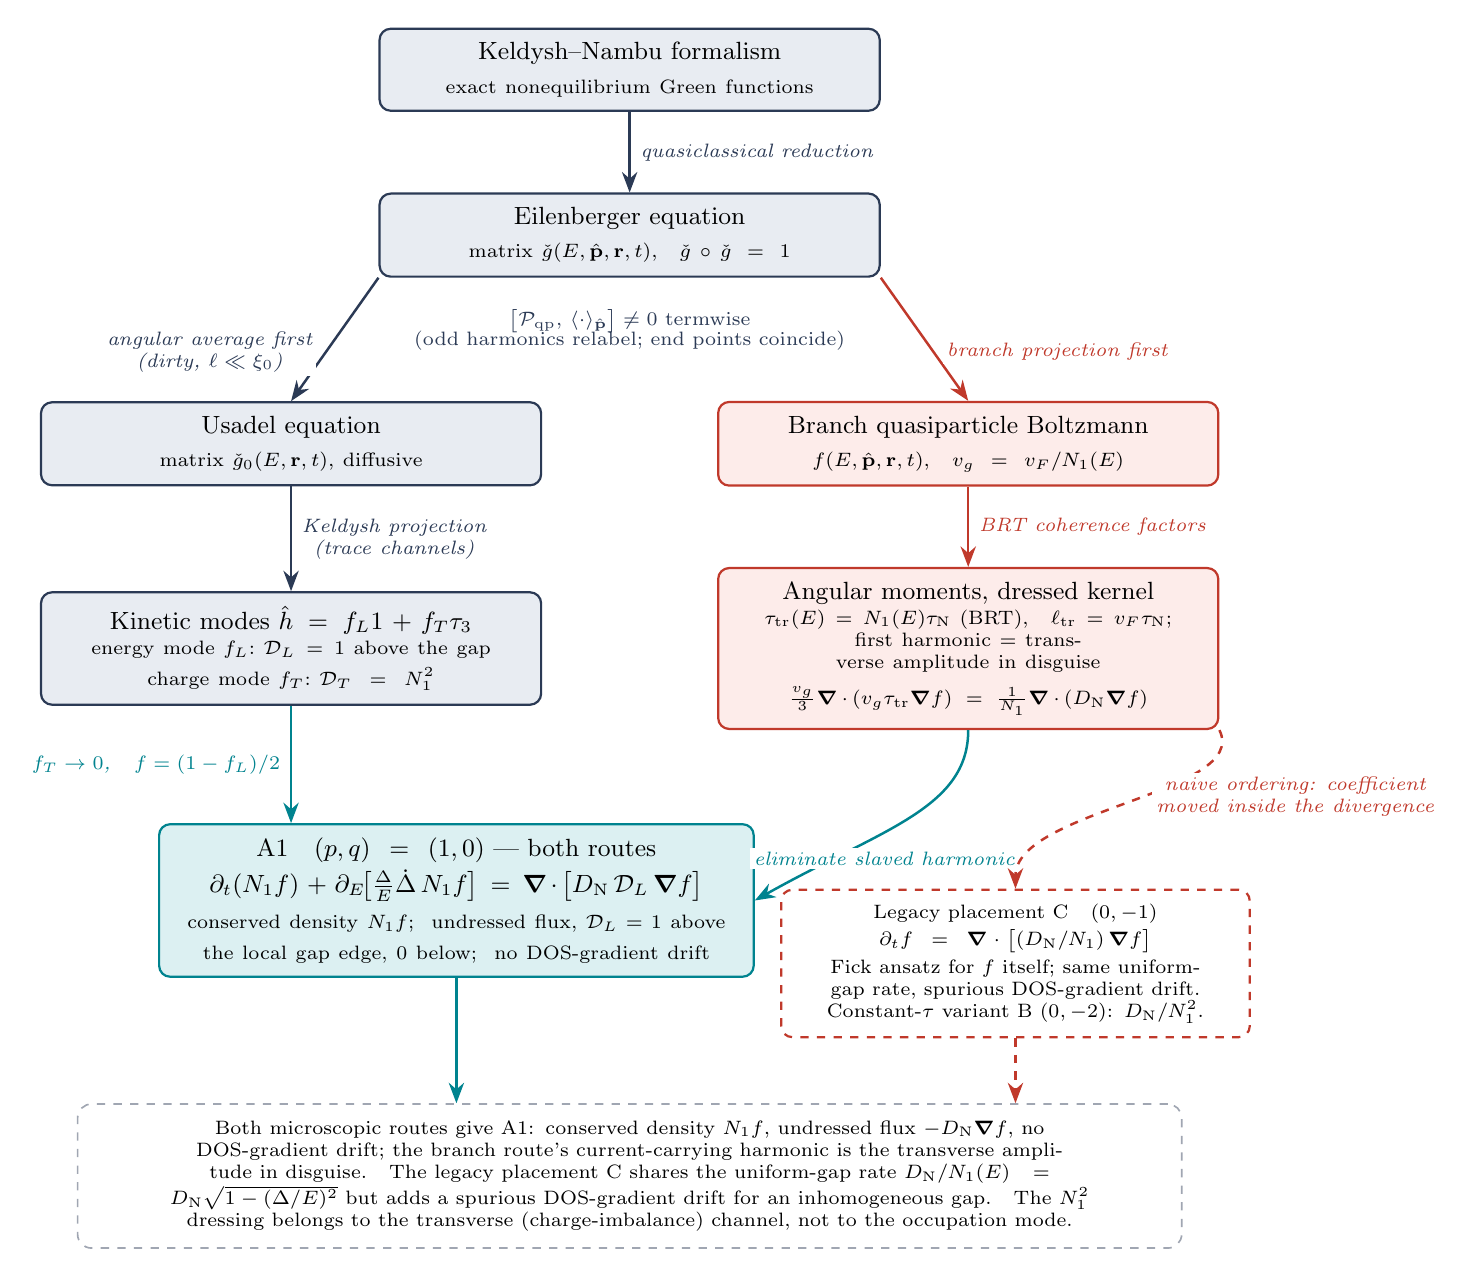
\begin{tikzpicture}

% ---------------- spine ----------------
\node[matrixbox] (keldysh) at (0,0)
  {Keldysh--Nambu formalism\\[1pt]
   {\scriptsize exact nonequilibrium Green functions}};

\node[matrixbox] (eilen) at (0,-2.1)
  {Eilenberger equation\\[1pt]
   {\scriptsize matrix $\check g(E,\hat{\mathbf p},\mathbf r,t)$,\quad
    $\check g\circ\check g=\id$}};

\draw[arr] (keldysh) -- node[lab,right=2pt]{quasiclassical reduction} (eilen);

% ---------------- the fork (termwise non-commuting, same end point) ----------------
\node[font=\scriptsize, text=slate, align=center] at (0,-3.30)
  {$\bigl[\mathcal P_{\mathrm{qp}},\,
    \langle\cdot\rangle_{\hat{\mathbf p}}\bigr]\neq 0$ termwise\\[-1pt]
   (odd harmonics relabel; end points coincide)};

\node[matrixbox] (usadel) at (-4.3,-4.75)
  {Usadel equation\\[1pt]
   {\scriptsize matrix $\check g_0(E,\mathbf r,t)$, diffusive}};

\node[branchbox] (branch) at (4.3,-4.75)
  {Branch quasiparticle Boltzmann\\[1pt]
   {\scriptsize $f(E,\hat{\mathbf p},\mathbf r,t)$,\quad
    $v_g=v_F/N_1(E)$}};

\draw[arr] (eilen.south west)
  -- node[lab, pos=0.60, left=3pt]
     {angular average first\\(dirty, $\ell\ll\xi_0$)} (usadel.north);
\draw[redarr] (eilen.south east)
  -- node[lab, pos=0.60, right=3pt]
     {branch projection first} (branch.north);

% ---------------- dirty route ----------------
\node[matrixbox] (modes) at (-4.3,-7.35)
  {Kinetic modes
   $\hat h=f_L\id+f_T\tau_3$\\[1pt]
   {\scriptsize energy mode $f_L$:\ $\mathcal D_L=1$ above the gap\\
    charge mode $f_T$:\ $\mathcal D_T=N_1^{2}$}};

\draw[arr] (usadel) -- node[lab,right=2pt]
  {Keldysh projection\\(trace channels)} (modes);

% ---------------- branch route ----------------
\node[branchbox] (slaving) at (4.3,-7.35)
  {Angular moments, dressed kernel\\[1pt]
   {\scriptsize $\tau_{\mathrm{tr}}(E)=N_1(E)\tau_{\mathrm{N}}$ (BRT),\quad
    $\ell_{\mathrm{tr}}=v_F\tau_{\mathrm{N}}$;\\
    first harmonic $=$ transverse amplitude in disguise\\[2pt]
    $\tfrac{v_g}{3}\boldsymbol\nabla\!\cdot\!
     (v_g\tau_{\mathrm{tr}}\boldsymbol\nabla f)
     =\tfrac{1}{N_1}\boldsymbol\nabla\!\cdot\!
      (\DN\boldsymbol\nabla f)$}};

\draw[redarr] (branch) -- node[lab,right=2pt]
  {BRT coherence factors} (slaving);

% ---------------- common end point ----------------
\node[resultbox] (aone) at (-2.2,-10.55)
  {A1\quad $(p,q)=(1,0)$ --- both routes\\[2pt]
   $\partial_t(N_1 f)+\partial_E\!\bigl[\tfrac{\Delta}{E}\dot\Delta\,
    N_1 f\bigr]=\boldsymbol\nabla\!\cdot\!\bigl[\DN\,\mathcal D_L\,
    \boldsymbol\nabla f\bigr]$\\[2pt]
   {\scriptsize conserved density $N_1 f$;\ \ undressed flux,
    $\mathcal D_L=1$ above the local gap edge, $0$ below;\ \
    no DOS-gradient drift}};

\draw[tealarr] (modes) -- node[lab,left=2pt]
  {$f_T\to 0$,\quad $f=(1-f_L)/2$} (aone.north -| modes);
\draw[tealarr] (slaving.south) .. controls +(0,-1.0) and +(1.6,0.9) ..
  node[lab, pos=0.60, below=5pt]
  {eliminate slaved harmonic}
  (aone.east);

% ---------------- legacy placement (not a route end point) ----------------
\node[legacybox] (cbox) at (4.9,-11.35)
  {Legacy placement C\quad $(0,-1)$\\[2pt]
   $\partial_t f=\boldsymbol\nabla\!\cdot\!\bigl[(\DN/N_1)\,
    \boldsymbol\nabla f\bigr]$\\[2pt]
   Fick ansatz for $f$ itself; same uniform-gap rate, spurious
   DOS-gradient drift.\\ Constant-$\tau$ variant B $(0,-2)$: $\DN/N_1^{2}$.};

\draw[reddash] (slaving.south east) .. controls +(0.4,-0.8) and +(0,1.0) ..
  node[lab, pos=0.45, right=2pt]
  {naive ordering: coefficient\\moved inside the divergence}
  (cbox.north);

% ---------------- punchline ----------------
\node[notebox] (note) at (0,-14.05)
  {Both microscopic routes give A1: conserved density $N_1f$, undressed
   flux $-\DN\boldsymbol\nabla f$, no DOS-gradient drift; the branch
   route's current-carrying harmonic is the transverse amplitude in
   disguise.\quad
   The legacy placement C shares the uniform-gap rate
   $\DN/N_1(E)=\DN\sqrt{1-(\Delta/E)^2}$ but adds a spurious DOS-gradient
   drift for an inhomogeneous gap.\quad
   The $N_1^{2}$ dressing belongs to the transverse (charge-imbalance)
   channel, not to the occupation mode.};

\draw[tealarr] (aone.south) -- (aone.south |- note.north);
\draw[reddash] (cbox.south) -- (cbox.south |- note.north);

\end{tikzpicture}
\end{document}
